% Shared standalone design for the editable figure reconstructions.
\documentclass[tikz,border=5pt,10pt]{standalone}
\usepackage[T1]{fontenc}
\usepackage[utf8]{inputenc}
\usepackage{newpxtext,newpxmath}
\usepackage[scaled=.94]{sourcesanspro}
\usepackage{pgfplots}
\pgfplotsset{compat=1.18}
\usetikzlibrary{arrows.meta,calc,positioning,decorations.pathreplacing,
  decorations.markings,patterns,matrix,shapes.geometric,fit,backgrounds,
  intersections,angles,quotes}
\definecolor{ink}{HTML}{203746}
\definecolor{accent}{HTML}{146C78}
\definecolor{muted}{HTML}{667780}
\definecolor{signalred}{HTML}{B94B44}
\color{ink}
\tikzset{>=Latex,line width=.8pt,
  every node/.style={font=\small},
  axis/.style={->,draw=muted,line width=.5pt},
  guide/.style={draw=muted,dashed,line width=.45pt},
  curve/.style={draw=accent,line width=1pt},
  marker/.style={circle,fill=accent,inner sep=1.5pt},
  labelbox/.style={fill=white,inner sep=2pt}}

\begin{document}
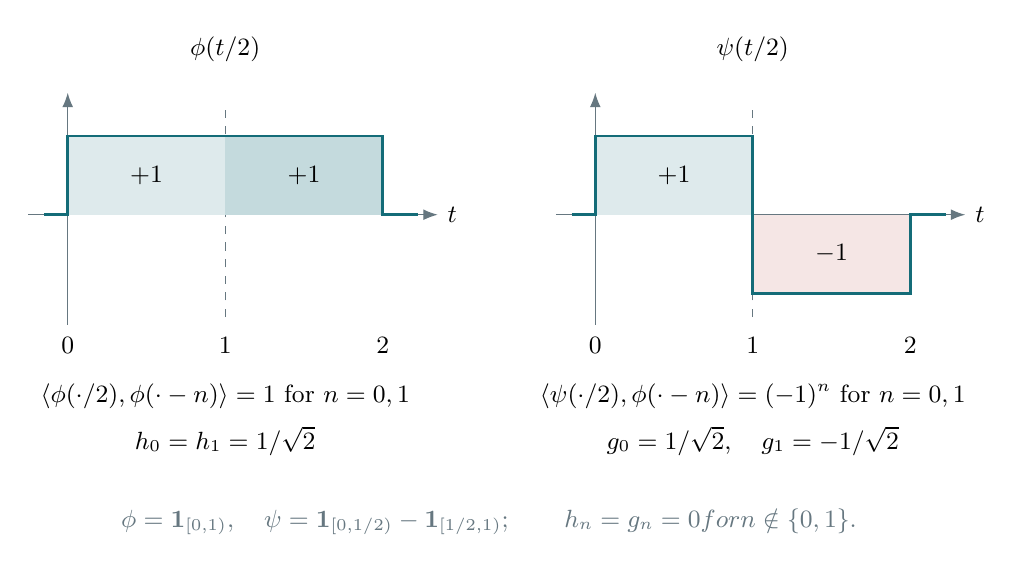
\begin{tikzpicture}[x=1cm,y=1cm]
\foreach \shift/\name in {0/{\phi(t/2)},6.7/{\psi(t/2)}}{\begin{scope}[shift={(\shift,0)}]
\draw[axis] (-.5,0)--(4.7,0) node[right] {$t$};
\draw[axis] (0,-1.4)--(0,1.55);
\foreach \x/\lab in {0/0,2/1,4/2}{\node[below] at (\x,-1.43) {$\lab$};}
\node at (2,2.1) {$\name$};
\draw[guide] (2,-1.3)--(2,1.35);
\end{scope}}
\fill[accent!14] (0,0) rectangle (2,1);\fill[accent!25] (2,0) rectangle (4,1);
\draw[curve] (-.3,0)--(0,0)--(0,1)--(4,1)--(4,0)--(4.45,0);
\node at (1,.5) {$+1$};\node at (3,.5) {$+1$};
\fill[accent!14] (6.7,0) rectangle (8.7,1);\fill[signalred!14] (8.7,0) rectangle (10.7,-1);
\draw[curve] (6.4,0)--(6.7,0)--(6.7,1)--(8.7,1)--(8.7,-1)--(10.7,-1)--(10.7,0)--(11.15,0);
\node at (7.7,.5) {$+1$};\node at (9.7,-.5) {$-1$};
\node[align=center] at (2,-2.6) {$\langle\phi(\cdot/2),\phi(\cdot-n)\rangle=1$ for $n=0,1$\\[6pt]$h_0=h_1=1/\sqrt2$};
\node[align=center] at (8.7,-2.6) {$\langle\psi(\cdot/2),\phi(\cdot-n)\rangle=(-1)^n$ for $n=0,1$\\[6pt]$g_0=1/\sqrt2,\quad g_1=-1/\sqrt2$};
\node[muted] at (5.35,-3.9) {$\phi=\mathbf1_{[0,1)},\quad\psi=\mathbf1_{[0,1/2)}-\mathbf1_{[1/2,1)};\qquad h_n=g_n=0\text{ for }n\notin\{0,1\}.$};
\end{tikzpicture}
\end{document}
